%!TEX root = ../dissertation.tex

\chapter{Thermalization in an isolated quantum~system}

Parts of this chapter have been published in the following publication:

\begin{quote}
	{Adam M. Kaufman, M. Eric Tai, Alexander Lukin, Matthew Rispoli, \\ Robert Schittko, Philipp M. Preiss, Markus Greiner} \\
	\textit{Quantum thermalization through entanglement in an isolated many-body system}\\
	\textit{Science} \textbf{353, 6301}, 794-800 (2016)
\end{quote}


\section{Statistical mechanics: from  classical to quantum}

Classical statistical mechanics relies on the notion of ensemble averaging \cite{Chandler1987}, which implies that the system occupies the entire phase space available to it. Since a classical system is in a single state of its phase space at any given point in time, in order to justify the assumptions of statistical mechanics we commonly rely on the ergodic hypothesis \cite{Penrose1970}. This assumption says that during the time evolution a system uniformly explores the entire available phase space. Ultimately, then, time averaging is said to be equal to ensemble averaging \cite{Penrose1970}. It's important to note here, that the ergodic hypothesis in such a setting implies thermalization only in a \textit{weak sense}, where weak refers to the fact that the statement is made only about \textit{time-averaged} values of observables after long times. In order to obtain thermalization in the \textit{strong sense}, namely in the sense that the \textit{instantaneous} values of observables at long times equal those predicted by thermodynamic ensemble, one has to consider classical chaotic systems like the Fermi-Ulam model \cite{Lichtenberg1992}, the Kapitza pendulum \cite{Broer2004}, and the kicked rotor \cite{Chirikov1979}.

At this point, one can ask how to translate the classical ideas of thermalization to the quantum language, in particular, whether a quantum system can have thermalization in the strong sense? At first glance, it seems elusive, since the evolution of a quantum system is governed by the Schr\"odinger equation, which is linear and thus cannot provide chaotic dynamics. However, recent theoretical breakthroughs \cite{Deutsch1991, Srednicki1994, Rigol2008} have shown that quantum systems also exhibit thermalization. These ideas rely on a conjecture named eigenstate thermalization hypothesis (ETH) \cite{Srednicki1999}, which states that in a chaotic quantum system individual eigenstates are thermal by nature. In order to understand the meaning of this statement, we first need to understand what exactly thermalizes in such systems.

\begin{figure*}[t]
	\centering
	\includegraphics[scale=1.5]{figures/ETH_fig1.pdf}
	\caption{{\bf Schematic of thermalization dynamics in closed systems}.  An isolated quantum system at zero temperature can be described by a single pure wave function $\vert \Psi \rangle$. Subsystems of the full quantum state appear pure, as long as the correlations (indicated by grey lines) between subsystems is negligible. If suddenly perturbed, the full system evolves unitarily, developing significant correlations between all parts of the system. While the full system remains in a pure, and in this sense zero-entropy state, the correlations between the subsystem and its complement drive local equilibration, and local, thermal mixed states appear to emerge within a globally pure quantum state.  }
	\label{fig:ETH_conceptual}
\end{figure*}

In the early days of quantum mechanics von Neumann noted that, when talking about thermalization, one should focus on local observables rather than wave functions, which carry all global properties of the system (see fig.~\ref{fig:ETH_conceptual}). This approach is very similar to a classical example of an isolated container with a gas, where we focus on a small volume inside the container to get a statistical ensemble for the subsystem. From this point of view, ETH can be formulated as following: Within a small energy window, in a quantum chaotic system the expectation value of a local observable is similar between the individual eigenstates and equal to microcanonical ensemble average. In more rigorous mathematical terms, ETH states that the matrix elements of a local observable $O_{nm}$ between eigenstates $\ket{n}$ and $\ket{m}$ can be effectively described as \cite{Srednicki1999}: 
\begin{equation}
O_{nm} = O(\bar{E}) \delta_{nm} + e^{-S(\bar{E})/2} f_O (\bar{E}, \omega) R_{nm},
\end{equation}
where $\bar{E} \equiv (E_n+E_m)/2$, $\omega \equiv E_n-E_m$ and $S(E)$ is thermodynamic entropy at energy $E$. Crucially, $O(E)$ and $f_O(E,\omega)$ are smooth functions of their arguments, the value $O(E)$ is identical to the expectation value of the microcanonical ensemble at energy $E$ and $R_{mn}$ is a random real or complex variable with zero mean and unit variance. One important remark should be made at this point: there are exceptions form this rule, namely the ground state and low-lying eigenstates as well as the states on top of the spectrum. Taking this into account, we say that ETH holds for the eigenstates in the middle of the spectrum. 

\section{Quench dynamics of an isolated quantum system}

Unfortunately, there is no known experimental technique to reliably prepare individual exited eigenstates many-body Hamiltonians. But since we are interested in dynamics associated with eigenstates in the middle of the spectrum we need to find a way to populate them. Here, quantum quenches come in handy. A quench is a sudden change in the Hamiltonian parameters, such that the wave function doesn't have time to adjust and, hence, gets reprojected onto the eigenstates of the new Hamiltonian (see fig.\ref{fig:ETH_quench}). In our experiments, we always start in the ground state of the initial Hamiltonian. The energy of this state lies well above the ground state of the final Hamiltonian and the state itself has very small overlap with any of the final eigenstates. Hence, the initial state gets projected onto a large superposition of states primarily in the middle of the spectrum of the final Hamiltonian. 

\begin{figure*}[t!]
	\centering
	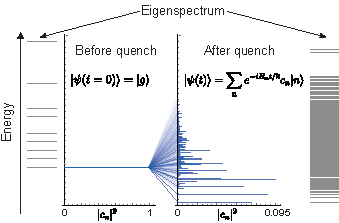
\includegraphics[scale=1.5]{figures/ETH_quench.pdf}
	\caption{{\bf Quantum quench.} The wave function of the system starting in the single state of the initial Hamiltonian gets reprojected onto a large number of different eigenstates after the sudden change in the system parameters. During the time evolution fallowing the quench the eigenstates dephase with respect to one another due to their energy mismatch. }
	\label{fig:ETH_quench}
\end{figure*}

After the quench, the time evolution of the state can formally be written in the basis of final Hamiltonian eigenstates $\ket{n}$ as
\begin{equation}
\ket{\psi(t)}=\sum_n e^{-iE_nt/\hbar}c_n\ket{n},
\end{equation}
where $E_n$ and $c_n$ are the corresponding energy and amplitude of the projection. Generally, this sum contains a large number of oscillating terms between the off-diagonal elements with large frequency, since the energy difference $E_n-E_m$ between adjacent eigenstates can be arbitrarily small. However, ETH predicts that, for a sufficiently local observable and states with large entanglement, the contribution of the off-diagonal terms is exponentially small. Hence the expectation value of such observables is determined only by the projection amplitudes $c_n$, after some transient evolution time. In addition, the expectation value for thermal eigenstates is equal to the microcanonical ensemble. Hence, if our state populates primarily eigenstates in the middle of the spectrum, its local observables will appear thermal.  

\section{Experimental protocol}
In our experiments, we study the emergence of thermalization in a six-site chain of interacting Bosons. To initiate the experiment, we isolate a $2 \times 6$ plaquette from a larger low-entropy Mott insulator with unity filling as shown in figure~\ref{fig:ETH_protocol}. At this point, each system is in a product state of single-atom Fock states on each of the constituent sites. We then suddenly switch on tunnelling along the chains while the tunnelling between them is suppressed. Each chain is restricted to the original six sites by introducing a barrier at the ends of the chains to prevent tunnelling out of the system. Each chain represents an identical but independent copy of a quenched system of six particles on six sites, which evolves in the quenched Hamiltonian for a controllable duration.

\begin{figure}[t]
	\centering
	\includegraphics[scale=1.2]{figures/ETH_protocol.pdf}
	\caption{{\bf Experimental sequence }. Using tailored optical potentials superimposed on an optical lattice. We deterministically prepare two copies of a six-site Bose-Hubbard system, where each lattice site is initialized with a single atom. We enable tunnelling in the x-direction and obtain either the ground state (adiabatic melt) or a highly excited state (sudden quench) in each six-site copy. After a variable evolution time, we freeze the evolution and characterize the final quantum state by either acquiring number statistics or the local and global purity.}
	
	\label{fig:ETH_protocol}
\end{figure} 

In the data that follow, we realize measurements of on-site number statistics and the quantum purity of the state. For measurements of the latter, we append to the quench evolution a beam splitter operation that interferes the two identical copies by freezing dynamics along the chain and allowing for tunnelling in a projected double-well potential for a prescribed time~\cite{Islam2015}. In the last step for both measurements, a potential barrier is raised between the two copies and a full counting procedure is performed to measure the resulting occupation on each site of each copy.

\section{Local observables in the thermalized pure state}
Recent experiments have demonstrated analogies between classical chaotic dynamics and the role of entanglement in few-qubit spin systems~\cite{Neill2016}, as well as the dynamics of thermalization within an ion system~\cite{Clos2016}. Furthermore, studies of bulk gases have shown the emergence of thermal ensembles and the effects of conserved quantities in isolated quantum systems through macroscopic observables and correlation functions~\cite{Trotzky2012,Langen2013,Geiger2014,Langen2015}.

In order to observe thermalization in our system, we first focus on measurements of atom number distributions in various subsystems of the chain. In figure~\ref{fig:ETH_Ensembles}B the number distribution for a single site and half of the chain is shown for two different final values of $U/J = 1.56$ and $U/J =0.38$. The data is averaged in the saturated regime over $5$ times between $10$ and $20\mathrm{ms}$, and the error bars are the standard deviation in the measured probabilities. We can already make an observation that the standard deviation of measured probabilities is small compared to their value, which indicates that the system is in a quasi-stationary state with small temporal fluctuations around the mean value- a characteristic of a thermal state.


\begin{figure*}[t]
	\centering
	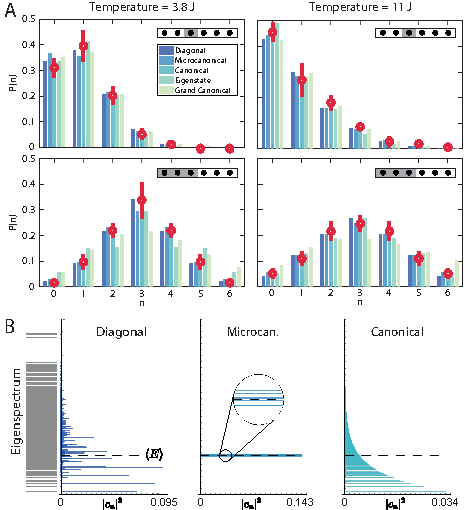
\includegraphics[scale=1.1]{figures/ETH_localDistr.pdf}
	\caption{{\bf Local observables in a quenched state. } {\bf (A)} Probability distribution of number operator is shown for subsystems of one and tree sites and for two different final quench depth. Along with the microcanonical ensemble, several other closely related ensembles are compared to the data. The error bars are the standard deviation of our observation over times between $10$ and $20\mathrm{ms}$. The measured number statistics are in excellent agreement with microcanonical and canonical thermal ensembles, verifying the thermal character of the local density matrix. {\bf (B)} Various thermal ensembles that were used for comparison with the data. The eigenspectrum of the final Hamiltonian along with initial projection amplitudes onto the many-body eigenstates are shown on the left.}
	\label{fig:ETH_Ensembles}
\end{figure*}

We compare our measurements to the predictions of thermal ensembles that are illustrated in Figure~\ref{fig:ETH_Ensembles}A, as well as a grand-canonical ensemble truncated to our total atom number~\ref{AppendixA}: this ensemble perhaps most closely models how well the many-body state can act as a reservoir for its constituent subsystems. The consistency within the error bars indicates that in this temporal range our observations remain near the thermal predictions despite the presence of temporal fluctuations. For the single site subsystem, the data is in good agreement with all the ensembles considered. Despite the fact that the quenched state is in a large distribution of eigenstates, we find favorable agreement for the case of a single eigenstate ensemble: this illustrates a key principle of ETH, which holds that expectation values of local observables vary slowly from eigenstate to eigenstate and are therefore relatively insensitive to the width of the distribution of populated states from the quench. We perform the same comparisons for the three-site case in the bottom two panels. Here we also observe agreement with most ensembles, though, interestingly, there is relatively less agreement with the single eigenstate and grand-canonical ensembles, particularly for the lower temperature quench. This variation in the agreement may suggest that these ensembles are more sensitive to the relative size of the reservoir compared to the subsystem, which indicates directions of further experiments~\cite{Rigol2012}.

\begin{figure*}[t!]
	\centering
	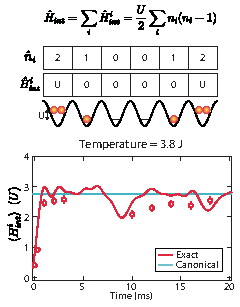
\includegraphics[scale=1.75]{figures/ETH_Eint.pdf}
	\caption{{\bf Interaction energy of the full system. } Thermalization occurs even for global quantities such as the full system interaction energy. The thermalization dynamics as calculated from our number-resolved images are in near agreement with exact numerical simulation and a canonical prediction.}
	\label{fig:ETH_Eint}
\end{figure*}

The above measurements were on specific subsystems, but our measurements also allow extraction of the average global interaction energy given by Hamiltonian:
\begin{equation}
\hat{H}_{int}=\frac{U}{2}\sum_i \hat{n}_i(\hat{n}_i-1),
\end{equation}
where $\hat{n}_i$ is the number operator on the $i\mathrm{-th}$ site and the summation runs over all sites of the chain (see fig.~\ref{fig:ETH_Eint}). Since the interaction Hamiltonian is diagonal in the Fock basis, we can use our measurements of the final particle configurations to compute the expectation value $\langle \hat{H}_{int} \rangle$. For the $T=3.8J$ data, we show a time scan indicating the initial growth in this quantity, which starts at zero since the initial state is a single particle per site.  These observations, at long times, are in near agreement with the canonical prediction. Interestingly, this measurement is sensitive to the entire six-site system as opposed to some subset of sites, which might suggest that it is global and unlikely to thermalize. Yet, $\langle \hat{H}_{int} \rangle$ undergoes thermalization because it is a sum of local operators, each of which thermalizes and is insensitive to the global purity of the full system.  The observed agreement is consistent with the idea that only a small set of operators, such as the global purity or other specific fine-tuned state projectors, can truly distinguish the pure state we produce from a thermal state.

\section{Thermalization of subsystem density matrix}

\begin{figure}[t]
	\centering
	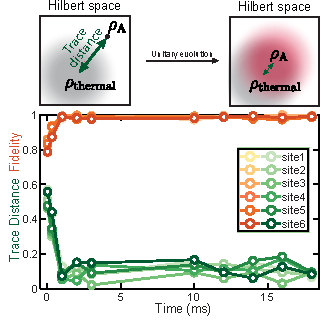
\includegraphics[scale=1.5]{figures/ETH_fidelity.pdf}
	\caption{{\bf Thermalization of the single-site density matrix.} In measuring the probabilities to observe a given particle number on a single site, we can obtain the local, single-site density matrix and observe the approach to thermalization. Using two different metrics, we compare the mixed state observed to the mixed state derived from the subsystem of a canonical thermal ensemble, after a quench to $U/J=1.56$. The trace distance provides an effective distance between the mixed states in Hilbert space, while the fidelity is an overlap measure for mixed states. The two metrics illustrate how the pure state subsystem approaches the thermal ensemble subsystem shortly after the quench. The starting value of these quantities is given by the overlap of the initial pure state with the thermal mixed state. Solid lines connect the data points.}
	\label{fig:ETH_Rho}
\end{figure} 

We can perform a more rigorous test of single-site thermalization by comparing the measured density matrix of each site with the reduced density matrix of a canonical thermal ensemble $\rho_A^T$ (Figure~\ref{fig:ETH_Rho}B). Our measurements of probabilities to observe a given particle number on a site completely characterize that single-site density matrix, because there are no coherences between different number states due to super-selection rules. With this measured density matrix, we can perform a quantitative comparison to a thermal ensemble using the trace distance ($\frac{1}{2}\mathrm{Tr}(\vert \rho_A^T -  \rho_A \vert)$) and quantum fidelity ($\mathrm{Tr}\left ( \sqrt{\sqrt{\rho_A^T} \rho_A \sqrt{\rho_A^T}}\right )$), both of which quantify the similarity of two mixed quantum states. After a short time, we see a quantum fidelity exceeding $99\%$ and a trace-distance that fluctuates between $0$ and $0.1$, indicating the similarity between the local density matrix of a verified pure state with the local density matrix of a thermal state. The correspondence between the observables of a pure state and thermal state depends on the equivalence of their reduced density matrices within the Hilbert space sampled by the observable. The measurement of Figure~\ref{fig:ETH_Rho}B therefore shows that observables for the single-site Hilbert space should agree with the predictions of thermal ensembles. 

\begin{figure}[t]
	\centering
	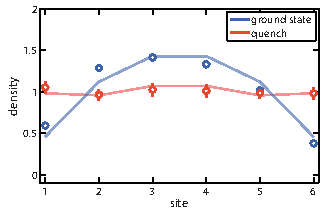
\includegraphics[scale=1.5]{figures/ETH_density.pdf}
	\caption{{\bf Local indistinguishability of a thermal state.} {\bf(A)} After quenching to $U/J=0.38$, the saturated average particle number on each site (density) is nearly equal among the sites of the system, which resembles a system at thermal equilibrium. By comparison, the ground state for the same Bose-Hubbard parameters has significant curvature.}
	\label{fig:ETH_density}
\end{figure} 

One consequence of single-site thermalization is that individual sites appear identical to one another. In a system with open boundary conditions, this is a striking contrast to the ground state, which is minimizing its energy. As an example, we look at the average particle number distribution in our system (see fig.~\ref{fig:ETH_density}). While the ground state exhibits significant curvature, corresponding to the ground state solution of the Shr\"odinger equation for a particle in the box., the quenched state exhibits a flat density distribution, manifesting the interchangeability of different sites of the system.

\section{Global state purity}

One straightforward consequence of the subsystem's density matrix being thermal is that the state of the subsystem is no longer pure. One potential explanation could be that during the time evolution that leads to thermalization the state as a whole couples to the environment and hence loses its global purity. In order to exclude this scenario, we measure the purity of our system during the time evolution.   

Tomography of the full quantum state would typically be required to extract the global purity, which is particularly challenging in the full 462-dimensional Hilbert space defined by the itinerant particles in our system. Furthermore, while in spin systems global rotations can be employed for tomography~\cite{Sackett2000}, there is no known analogous scheme for extracting the full density matrix of a many-body state of itinerant particles. The many-body interference described here, however, allows us to extract quantities that are quadratic in the density matrix, such as the purity~\cite{Islam2015}. After performing the beam splitter operation, we can obtain the quantum purity of the full system and any subsystem simply by counting the number of atoms on each site of one of the six-site chains. Each run of the experiment yields the parity $P^{(k)} = \Pi_i p^{(k)}_i$, where $i$ is iterated over a set of sites of interest in copy-$k$. The single-site parity operator $p^{(k)}_i$ returns 1 (-1) when the atom number on site-$i$ is even (odd). It has been shown that the beam splitter operation yields $\langle P^{(1)} \rangle = \langle P^{(2)} \rangle = \mathrm{Tr}\left (\rho_1 \rho_2  \right)$, where $\rho_i$ is the density matrix on the set of sites considered for each copy~\cite{Palmer2005, Daley2012,Islam2015}. Because the preparation and quench dynamics for each copy are identical, yielding $\rho_1 = \rho_2 \equiv \rho$, the average parity reduces to the purity: $\langle P^{(k)} \rangle = \mathrm{Tr}(\rho^2)$. When the set of sites considered comprises the full six-site chain, the expectation value of this quantity returns the global many-body purity, while for smaller sets it provides the local purity of the respective subsystem.

\begin{figure}[t]
	\centering
	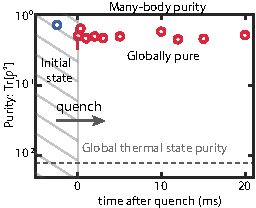
\includegraphics[scale=2]{figures/ETH_purity.pdf}
	\caption{{\bf Verifying global state purity}  We can measure the global many-body purity, and observe a static, high purity. This is in stark contrast to the vanishing global purity of the canonical thermal ensemble, yet this same ensemble accurately describes the local number distribution we observe.
	}
	\label{fig:ETH_purity}
\end{figure}

We find that the global many-body state retains its quantum purity during the entire time of our experiment, affirming the unitarity of its evolution following the quench (see. fig.~\ref{fig:ETH_purity}). This global measurement also clearly distinguishes the quantum state we produce from a canonical thermal ensemble, we used to describe the local observables in our system, as the purity between the two is different by two orders of magnitude. The deviation of the global state purity from unity can be explained by non-perfect beamsplitter fidelity in our system due to the residual interaction between the particles.

\section{Entanglement in a quantum system}
One of the defining concepts of quantum mechanics is the superposition principle, which allows the system to be in multiple states at the same time. This can lead to the formation of correlations that go beyond classical local theories \cite{Horodecki2009}. The most famous example is a Bell state \cite{Bell1964}, which can be written in the context of two spin $\frac{1}{2}$ particles as 
\begin{equation}
\left| \psi \right>=(\left| \uparrow \downarrow \right>+ \left| \downarrow \uparrow \right>)/\sqrt{2},
\end{equation}
where up and down arrows represent one of the two states of each spin. The remarkable property of this state is that no matter which basis one would choose to measure the spin of both particles, the results of the measurement will always be anti-correlated. These basis independent correlations are called entanglement.

For a many-body system, it can be a formidable task to find all possible correlations that exist between its subsystems. To overcome this complication, we rely on the property of the entangled states, that ignoring the information about one subsystem puts the other into a classical mixture of states. The number of states in this mixture can be quantified by the purity of the subsystem's density matrix $\rho$, given by $\textrm{Tr}(\rho^2)$. If the state is pure $\textrm{Tr}(\rho^2)=1$, whereas for a mixed state $\textrm{Tr}(\rho^2)<1$.

\begin{figure}[t!]
	\centering
	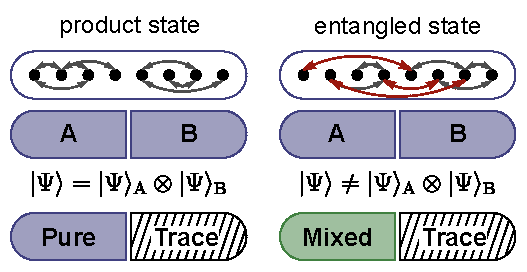
\includegraphics[scale=1]{figures/ETH_entanglemet.pdf}
	\caption{{\bf Entanglement and purity }. For a globally pure state the purity of the subsystem is related to the entanglement (represented by arrows) between the subsystems. If subsystems A and B are not entangled the full state is a tensor product of pure states of the subsystems. Therefore each of them remain pure if the information about the other one is ignored. Contrary, when A and B are entangled, the subsystems purity is decreased upon tracing, as the correlations between A and B are ignored in the reduced density matrix }
	\label{fig:ETH_entanglemet}
\end{figure}  

Consider and example of a globally pure state $\ket{\psi_{AB}}$ that is split into two subsystems A and B (see fig~\ref{fig:ETH_entanglemet}). Ignoring the information of one of the subsystem is equivalent to tracing the full system density matrix $\rho = \ket{\psi_{AB}}\bra{\psi_{AB}}$ with respect to the degrees of freedom of the ignored subsystem, for example $\rho_A =\textrm{Tr}_B(\rho)$. In case subsystems A and B are not entangled the full state is a tensor product of pure states of the subsystems $\ket{\psi_{AB}}=\ket{\psi_{A}}\otimes\ket{\psi_{B}}$. Hence $\rho_{A}= \ket{\psi_{A}}\bra{\psi_{A}}$ and $\rho_B= \ket{\psi_{B}}\bra{\psi_{B}}$, therefore $\textrm{Tr}(\rho_A^2)=\textrm{Tr}(\rho_B^2)=1$. For an entangled state, the subsystems are less pure than the full system as the correlations between A and B are ignored in the reduced density matrix, $\textrm{Tr}(\rho_A^2)=\textrm{Tr}(\rho_B^2)<1$.

Even if the full many-body state is mixed ($\textrm{Tr}(\rho_{AB}^2) < 1$), it is still possible to measure entanglement between the subsystems \cite{Horodecki2009}. It is sufficient \cite{Horodecki1996} to prove this entanglement by showing that the subsystems are less pure than the full system, i.e.
\begin{equation}
\begin{aligned}
&\textrm{Tr}(\rho_{A}^2)<\textrm{Tr}(\rho_{AB}^2)    \\
&\textrm{Tr}(\rho_{B}^2)<\textrm{Tr}(\rho_{AB}^2)
\end{aligned}
\end{equation}
These inequalities provide a tool for detecting entanglement in the presence of experimental imperfections. Furthermore, quantitative bounds on the entanglement present in a mixed many-body state can be obtained from these purities \cite{Mintert2007}.

A common measure of the entropy both in the classical and quantum case is the von Neumann entropy, defined with respect to the density matrix $\rho$ as:
\begin{equation}
S_{vN} = - \textrm{Tr}[\rho \textrm{Log}(\rho)],
\end{equation}
However, in our experiments we quantify the entanglement using the second-order R\'{e}nyi entropy $S_A = -\textrm{Log}(\textrm{Tr}[\rho_A^2])$, which is the logarithm of the purity of the subsystem density matrix. While the von Neumann entropy is typically used in the context of statistical mechanics, both quantities grow as a subsystem density matrix becomes mixed and increasingly entropic. In the R\'{e}nyi case, the purity in the logarithm quantifies the number of states contributing to the statistical mixture described by the density matrix. 

It is important to note that the thermodynamic relations in statistical mechanics, defined with the
von Neumann definition, do not directly apply for the R´enyi definition. However, R\'{e}nyi entropy provides a lower bound to the von Neumann entropy and is directly accessible by our measurements.

\section{Entanglement entropy dynamics after quench}
The growth of entanglement following a quench is key to understanding how entropy forms within the subsystems of a pure quantum state, thereby facilitating thermalization~\cite{Calabrese2005, Daley2012, Schachenmayer2013, Hazzard2014}. We study the dynamics of the entanglement entropy, for varying subsystem sizes (Figure~\ref{fig:EEDyn}). Initially, we observe an approximately linear rise in the entropy, with similar slope among the subsystems considered (Figure~\ref{fig:EEDyn} inset)~\cite{Calabrese2005}. After an amount of time that depends on the subsystem size, the entanglement entropy saturates to a steady-state value, about which there are small residual temporal fluctuations. The presence of residual fluctuations is, in part, attributable to the finite-size of our system. An exact numerical calculation of the dynamics with no free parameters shows excellent agreement with our experimental measurements. Crucially, the data indicate that while the subsystems acquire entropy in time (Figure~\ref{fig:EEDyn},A-C), the full system entropy remains constant and is small throughout the dynamics (Figure~\ref{fig:EEDyn}D). The high purity of the full system allows us to conclude that the dynamical increase in entropy in the subsystems originates in the propagation of entanglement between the system's constituents. 

\begin{figure*}[t!]
	\centering
	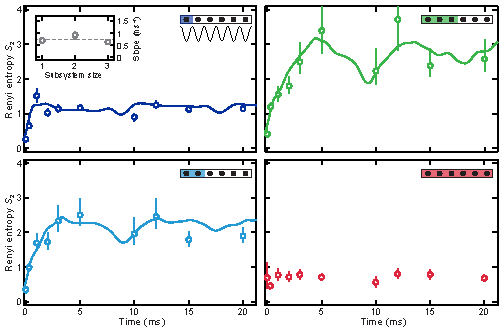
\includegraphics[scale=1.5]{figures/ETH_EE_dynamics.pdf}
	\caption{{\bf Dynamics of entanglement entropy. } Starting from a low-entanglement ground state, a global quantum quench leads to the development of large-scale entanglement between all subsystems. We quench a six-site system from the Mott insulating product state ($U/J\gg 1$) with one atom per site to the weakly interacting regime of $U/J=1.56$ ($J/(2\pi) = 66\mathrm{Hz}$) and measure the dynamics of the entanglement entropy. As it equilibrates, the system acquires local entropy while the full system entropy remains constant and at a value given by measurement imperfections. The dynamics agree with exact numerical simulations with no free parameters (solid lines), that are offset for all the subsystems by the amount of extensive entropy present in the state (see appendix~\ref{AppendixC}). Error bars are the standard error of the mean (S.E.M.). For the largest entropies encountered in the three-site system, the large number of populated microstates leads to a significant statistical uncertainty in the entropy, which is reflected in the upper error bar extending to large entropies or being unbounded. Inset: slope of the early time dynamics, extracted with a piecewise linear fit. The dashed line is the mean of these measurements.}
	\label{fig:EEDyn}
\end{figure*} 

The approximately linear rise at early times (Figure~\ref{fig:EEDyn} inset) is related to the spreading of entanglement in the system within an effective light cone~\cite{Calabrese2005,Cheneau2012,Richerme2014}. Furthermore, in analogy to the growth of the thermodynamic entropy in an equilibrating classical mechanical system, such as a gas in a closed container, we observe the growth of local entropy in a closed quantum mechanical system. In the quantum mechanical case, however, the mechanism responsible for entropy is entanglement, which is absent from a system modeled by classical mechanics.

\section{Correspondence between entanglement and thermal entropy}

When a system thermalizes, we expect that the saturated values of local observables should correspond to the predictions of a statistical ensemble. By analogy, if the entanglement entropy plays the role of thermal entropy, then in a thermalized pure state we expect extensive growth in the entanglement entropy with subsystem volume. This is called as a volume law. Ground-breaking theoretical work using conformal field theory has shown that indeed, at long times, a volume law is expected for a quenched, infinite, continuous system, while only an area law with a log correction is expected for the ground state~\cite{Calabrese2004, Calabrese2005, Rivas2010}. Characterizing the large amount of entanglement associated with a volume law is particularly challenging because it results in nearly every entry of the density matrix having small, but importantly non-zero magnitude. 

Using the techniques outlined in this work, we show measurements displaying a near volume law in the entanglement entropy (Figure~\ref{fig:volume}A). A linear growth with volume in the entanglement entropy occurs when each subsystem incoherently populates a number of states that scales with the size of the subsystem Hilbert space. This is because, for the Bose-Hubbard model, the Hilbert space is approximately exponential in the lattice size, which results in a linear growth in $S_A = -\textrm{Log}(\textrm{Tr}[\rho_{A}^2])$. Furthermore, the exact slope of the entanglement entropy versus subsystem volume depends on the average energy of the thermalized pure state~\cite{Garrison2015}. By contrast, we can prepare the ground state of the quenched Hamiltonian by adiabatically reducing the lattice depth. Here, the superfluid ground state of the Bose-Hubbard model has suppressed entanglement, which is predicted to incur slow logarithmic growth in the entanglement entropy with subsystem volume~\cite{Calabrese2004}. Our measurements clearly distinguish the two cases. The back-bending of the entanglement entropy as the subsystem surpasses half the system size indicates that the state is globally pure. In the quenched state, the high global purity is striking in a state that locally appears completely dephased, which is behaviour often associated with environmentally-induced decoherence or other noise sources. 

\begin{figure}[t]
	\centering
	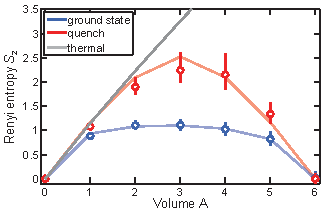
\includegraphics[scale=1.5]{figures/ETH_volumeLaw.pdf}
	\caption{{\bf Entanglement scaling. } After the quench, the many-body state reaches a thermalized regime with saturated entanglement entropy. In contrast to the ground state, for which the R\'{e}nyi entropy only weakly depends on subsystem size, the entanglement entropy of the saturated, quenched state grows almost linearly with size. As the subsystem size becomes comparable to the full system size, the subsystem entropy bends back to near zero, reflecting the globally pure zero-entropy state. For small subsystems, the R\'{e}nyi entropy in the quenched state is nearly equal to the corresponding thermal entropy from the canonical thermal ensemble density matrix. Throughout this figure, the entanglement entropies from the last time point in fig.~\ref{fig:EEDyn} are averaged over all relevant partitionings with the same subsystem volume; we also correct for the extensive entropy unrelated to entanglement. All solid lines are theory with no free parameters.}
	\label{fig:volume}
\end{figure}

We further observe quantitative agreement between the exact dependence of the entanglement entropy with subsystem volume and the prediction of a thermal ensemble. We make this comparison by computing a canonical thermal ensemble $\rho^T$ with an average energy that is the same as the quenched quantum state produced experimentally~\cite{Garrison2015}. The grey line in Figure~\ref{fig:volume}A is the R\'{e}nyi (thermal) entropy as a function of subsystem size for this calculated thermal state. Although our limited system size prevents comparison over a large range of subsystem sizes, the initial rise of the entanglement entropy with subsystem volume mimics that of the thermal entropy. Despite their similarity, it is worth emphasizing the disparate character of the thermal and entanglement entropy. The entanglement entropy (either the R\'{e}nyi or von Neumann) is instantaneously present in the pure quantum state after coherent unitary evolution, arising from the non-separability of the quantum state between the subsystem and traced out degrees of freedom. On the other hand, the von Neumann thermal entropy within a subsystem of a mixed thermal state is the thermodynamic entropy in statistical mechanics, which could be extracted from irreversible heat flow experiments on the subsystem~\cite{Deutsch2013}. Therefore, the similarity of the R\'{e}nyi  entropies we observe points to an experimental equivalence between the entanglement and thermodynamic entropy~\cite{Garrison2015,Grover2015}.

\begin{figure}[t]
	\centering
	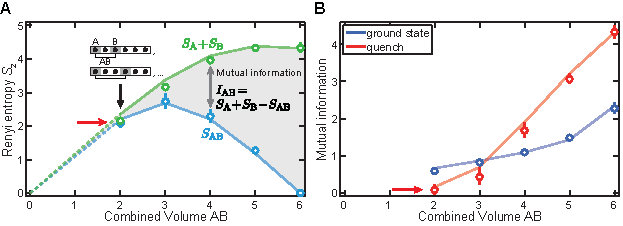
\includegraphics[width=140mm]{figures/ETH_MI.pdf}
	\caption{{\bf Mutual information in the thermal state. } {\bf (A)} The mutual information $I_{AB} = S_A + S_B - S_{AB}$ quantifies the amount of classical (statistical) and quantum correlations between subsystems A and B. For small subsystems, the thermalized quantum state has $S_A + S_B \approx S_{AB}$ due to the near volume law scaling (red arrow), leading to vanishing mutual information. When the volume of $AB$ approaches the system size, the mutual information will grow because $S_A + S_B$ exceeds $S_{AB}$. {\bf (B)} We study $I_{AB}$ vs the volume of AB for the ground state and the thermalized quenched state. For small system sizes, the quenched state exhibits smaller correlations than the adiabatically prepared ground state and is nearly vanishing. When probed on a scale near the system size, the highly entangled quenched state exhibits much stronger correlations than the ground state. Throughout this figure, the entanglement entropies from the last time point in fig.~\ref{fig:EEDyn} are averaged over all relevant partitionings with the same subsystem volume; we also correct for the extensive entropy unrelated to entanglement. All solid lines are theory with no free parameters.}
	\label{fig:MI}
\end{figure} 

The behaviour of the entanglement entropy provides a clear framework for understanding the entropy within thermalizing, closed quantum systems. However, one of the most famous features of entanglement, the presence of non-local correlations, appears inconsistent with what one expects of thermalized systems. In particular, the massive amount of entanglement implied by a volume law suggests a large amount of correlation between disparate parts of the system, while a key feature of a thermal state is the very absence of these long-range correlations. A useful metric for correlations, both classical (statistical) and quantum, between two subsystems $A$ and $B$ is the mutual information $S_A +S_B - S_{AB}$~\cite{Wolf2008, Islam2015}. The mutual information demonstrates that the amount of correlation in the presence of a volume law is vanishing for subsystem volumes that sample less than half the full system, which is where the entropy growth is nearly linear (Figure~\ref{fig:MI}). Furthermore, even though the thermalized quantum state carries more entanglement entropy than the ground state, small subsystems display smaller correlations than in the superfluid ground state. Once the subsystem volume is comparable to the system size, which is where the entanglement entropy deviates from the volume law, the quantum correlations entailed by the purity of the full system become apparent (Figure~\ref{fig:MI}B). The mutual information, therefore, illustrates how the volume law in the entanglement entropy yields an absence of correlations between sufficiently local observables, even though the quantum state retains a large amount of entanglement. 

\section{Conclusions}
In this chapter we have shown how a subsystem of a pure many-body state, undergoing quantum unitary dynamics, dynamically looses it's purity through entanglement with the rest of the system. This leads to the thermalization of the subsystem. We also show the correspondence between the classical thermal entropy and quantum entanglement entropy in the system. Our observations speak to a natural translation between thermalizing quantum and classical systems.

Classical statistical mechanics relies on a fundamental assumption: a system in thermal equilibrium can be found in any microstate compatible with the thermodynamic constraints imposed on the system, and, as such, is described by an ensemble of maximal entropy~\cite{Ma1985}.  Although it is vastly successful, classical statistical mechanics does not itself justify this entropy maximization for closed systems~\cite{Ma1985, Dalessio2016}, and an open systems approach only defers the question of thermalization to the union of the bath and system~\cite{Deutsch1991}. While ergodicity and time-averaging can provide a justification for entropy maximization in closed classical mechanical systems, ergodicity is not applicable on the same scale that statistical mechanics is successful, and time-averaging can require exponentially long times~\cite{Ma1985, Dalessio2016}. The latter also obscures the fact that there is in reality only one system, which, nevertheless, is  well-modeled by an entropic ensemble~\cite{Ma1985}. Our studies, and beautiful recent theoretical work~\cite{Rigol2012, Deutsch2013,Garrison2015}, hint towards a microscopic origin for entropy maximization in a single quantum state, namely that induced by the entanglement we measure.